
%%%%%%%%%%%%%%%%%%%%%%% file typeinst.tex %%%%%%%%%%%%%%%%%%%%%%%%%
%
% This is the LaTeX source for the instructions to authors using
% the LaTeX document class 'llncs.cls' for contributions to
% the Lecture Notes in Computer Sciences series.
% http://www.springer.com/lncs       Springer Heidelberg 2006/05/04
%
% It may be used as a template for your own input - copy it
% to a new file with a new name and use it as the basis
% for your article.
%
% NB: the document class 'llncs' has its own and detailed documentation, see
% ftp://ftp.springer.de/data/pubftp/pub/tex/latex/llncs/latex2e/llncsdoc.pdf
%
%%%%%%%%%%%%%%%%%%%%%%%%%%%%%%%%%%%%%%%%%%%%%%%%%%%%%%%%%%%%%%%%%%%


\documentclass[runningheads,a4paper]{llncs}

\usepackage{amssymb}
\setcounter{tocdepth}{3}
\usepackage{graphicx}
\usepackage{epstopdf}
\usepackage{subfig}
\usepackage{url}
\urldef{\mailsa}\path|{alfred.hofmann, ursula.barth, ingrid.haas, frank.holzwarth,|
\urldef{\mailsb}\path|anna.kramer, leonie.kunz, christine.reiss, nicole.sator,|
\urldef{\mailsc}\path|erika.siebert-cole, peter.strasser, lncs}@springer.com|
\newcommand{\keywords}[1]{\par\addvspace\baselineskip
\noindent\keywordname\enspace\ignorespaces#1}

\usepackage{todonotes}
\newcommand{\yongli}{\todo[author=YL,color=green,inline]}
%\newcommand{\naoki}{\todo[author=NK,color=yellow,inline]}

\newcommand{\eat}[1]{}
\begin{document}

\mainmatter  % start of an individual contribution

% first the title is needed
\title{Change Detection From Media Sharing Community }

% the name(s) of the author(s) follow(s) next
%
% NB: Chinese authors should write their first names(s) in front of
% their surnames. This ensures that the names appear correctly in
% the running heads and the author index.
%
\eat{
\author{Naoki Kito
\and Dr.Xiangmin Zhou\and Assoc Prof. James Thom}
}
\maketitle


\begin{abstract}
From ancient time, the damages or the destructions to the countries caused by the natural disasters were the major issues. 
Recently, through the improvement of image change detection technologies, social media and the high-resolution images, the damages caused by natural disasters can be analysed in more details to identify the situations in the cities or towns. Many researchers approached to analyse the damage by using the aerial images and the satellites images, but these images are often published to the public after the things settle down. However, when the disasters happen, people want the information of disasters as soon as possible. This research proposes to investigate how the social media images and the image change detection techniques can be used to identify the damages caused by the natural disasters. We first propose a framework that takes advantages of fast clustering and image near duplicate identification for the change detection in disasters. Then we model the social images by exploiting the image tags and location information. Following that, we propose a recursive 2 means algorithm over the new data model, and refine the changes by local interest point-based similarity matching. Finally, we propose a boundary representation model called \textit{relative position annulus} (RPA), which is robust to boundary oration, location shift and editing operations. A RPA matching approach is proposed by extending the dynamic time warping (DTW) measure from series to annulus. Extensive experiments have been done to evaluate the high effectiveness and efficiency of our approach.
\end{abstract}


\section{Introduction}

Before, during and after the natural disasters, information about the damages and the current situations are vital for people to make decisions for their next actions. For example, the Nepal earthquake in 2015 did a huge damage to everything, including buildings, roads, infrastructure, and people, which resulted in 8,019 people died and 17,866 people injured; in a Tokyo earthquake, people are still able to walk back home since the earthquake damage the infrastructure, but not the buildings and paths. A recent study \cite{110009470680} found that people would like to know earthquake size and epicentre.
Moreover, knowing these information could prevent the secondary and tertiary disasters. It is also found that in Tokyo, only 67.8\% of people managed to get back their house on the day of an earthquake, and the rest 32.2\% had to become ``\emph{homeless}", among them 2\% failed to going back home only because they could not find the safe path. People want the information about earthquakes, but there is always the question ``How should the people get the information of earthquakes?".

Recently, there are lots of researchers had approached to detect the damages caused by the natural disasters by using the change detection techniques with the aerial images. However, the aerial images consume longer times retrieve and harder to get compare to the other images. On the other hand, social media is pervasive, and updates very quickly especially on large events, e.g. natural disasters, by millions of people all the time. Thus, we investigate the problem of change detection from social media images, so as to let the public aware of the latest situations of natural disasters on the spot. One of the challenges here is the large-scale of the social media images, which makes current change detection techniques infeasible if not impossible. One of the limitation of using the large-scale images with current change detection techniques is the time cost. As existing techniques detect changes based on pixel level comparison \cite{ilsever2012two} without index support or query optimization or both, the time cost for image comparison is high. When applying them to large scale social images, the efficiency issue becomes even unacceptable. Another challenge is the unavailability of some special features, like building shady, used in traditional change detection approaches \cite{turker2008building}. In sharing communities, most of social images do not have shady, thus the shady-based matching can not be conducted. Forcing the existing techniques on the social images will cause low detection quality. Finally, traditional change detection over aerial images suppose the image pairs to the same location points are known, which is not true in media sharing communities.

\eat{\yongli{Explain why time cost is a issue for them?}
Another limitation is the unstable/unrelated images.
The social media image features are made by the up-loader and
this human inputs make the unstable/unrelated images.
\yongli{are we solving this?}
The image rotation, resolution and the quality of the images also the concern of the limitation.
}
%In this research, we target to detect the damages to the infrastructures and buildings, and this project investigates image change detection techniques and the social media images.

%In order to successfully support these tasks, the images from the social media have to cluster with the proper groups to make sure the gathered images are relevant to the natural disasters. Furthermore, the change detection system should be able to detect the damages of buildings and the roads.

%Our approach is to find the relevant images from the social media will be the Social Media Image Similarity, which is the combination of the Jaccard Similarity and the Location Similarity. Then, the images will be clustered by the Recursive 2-Means  algorithm \cite{1017616}. Finally, we are using a PCA-SIFT algorithm to match the before and the after images and find the changes between the images.
%In this paper, there are three alternative approaches to solve the questions. Firstly, the Jaccard Keywords Similarity \cite{Jaccard} is used to find the similarity between the user inputs and the tags(image tags, titles/topics and time) on the social media images. This will group or limit the images to a certain extent. Secondly, the Location Distance Similarity makes the groups of images more relevant to the natural disasters, by determine the location of the disaster happens.
%At the end of the clustering, it uses the PCA-SIFT to match before and after the disaster images.

To address these issues, we propose a framework for change detections in sharing communities. First, we represent the metadata of each image as a set of weighted tags, and propose a Social Image Similarity function ($SIS$) over image metadata and location. 
Then, we extend the recursive 2-means clustering algorithm \cite{} \yongli{Should we add this citation now?} from vector space in $L_p-norm$ to key word set space, so Jaccard-based $SIS$ measure can be applied. By deploying this extended recursive 2-means clustering over the whole image dataset, a number of small clusters are generated. Images in the same cluster or neighboring clusters will have the high probability of being the image pairs of the sources. Following that, we conduct PCA-SIFT based matching, which determines if two images are really referring to the same source. Finally, we propose a robust boundary representation that is robust to the view point rotation and other global transformations of the same objects in different images. Based on this representation, the boundary matching between image pair candidates is performed, which decides if a change has happened after disaster.

\eat{
we deploy existing clustering technique before using the change detection methods to detect the changes.
By applying the clustering methods to the large-scale image datasets,
we are able to retrieve the related images from the clustered images for the change detection.
Only applying the change detection method to the related images should increase the time performance and the accuracy of the change detection.
We use the Recursive 2 Means clustering and the new feature, Social Image Similarity is proposed for the data sets of the clustering.  The SIS is the total similarity between the images and it is the combination of the Tags Jaccard Similarity and the Locations Similarity.
The tags are the texture data which present what the images contain and the locations are the place where the images are upload to the social media.
Finally, we are using the PCA-SIFT algorithm to find the image similarities.


\yongli{It is still too detailed. I think a highlevel summarization about your technique would be better. After that, maybe one/two sentences for the details, but not too detailed.}
}

The contributions of this study are as follows:
\begin{itemize}
\item We propose a new similarity function $SIS$ over weighted tags and location of social images, and extend the recursive 2-means clustering for $SIS$ similarity. \eat{New Feature Social Image Similarity}
\item We perform PCA-SIFT-based matching which identifies the image pairs from the same object source. \yongli{I suggest to remove this from the contribution, as it is just the application of PCA-SIFT. ;) }
\item We propose a robust boundary representation model, based on which the boundary matching between images is conducted to identify the changes happened in disasters.
\item Extensive experiments have been conducted over large real social image data collection to evaluate the effectiveness and efficiency of our change detection system.
\end{itemize}

\eat{\yongli{Please list the contributions here}}

The rest of the paper is structured as follows: Section~\ref{sec-bg} reviews the related work; Section~\ref{sec-framework} presents the framework proposed in this study; Section~\ref{sec-datamodelling} details the modelling of the social media data; Section~\ref{sec-algorithm} presents the proposed change detection algorithm; Section~\ref{sec-evaluation} includes the experiment evaluation; Section~\ref{sec-con} concludes the paper.

\section{Related Work}\label{sec-bg}

In this section, we review the existing research closely related to this work, including the image copy detection and change detection.

\subsection{Image Copy Detection} \label{sec:ImageCopyDetection}
Image copy detection identifies the images of the same sources. Typically, image copy detection is done by first extracting the descriptors of local interest points in each image, and counting the number of matched descriptors between two compared ones. Examples on image descriptors include SIFT\cite{790410}, PCA-SIFT\cite{1315206}, SURF\cite{bay2006surf}, GLOH\cite{10.1109/TPAMI.2005.188}, and Eff$^2$\cite{DBLP:conf/mm/LejsekAJA06a} etc. In \cite{790410}, Lowe invented SIFT descriptor to find the similarity between images. The SIFT descriptor is extracted by four steps: scale-space extrema selection, keypoint localization, orientation assignment, and keypoint descriptor computation. First, scale-space extrema selection finds the ``interest points" in the image by using the Difference-of-Gussian Function(DoG). Then, by keypoint localization, the number of interest points is minimized and noise points are reduced. After that, the orientation assignment find the orientation of the images to ensure the invariance of descriptors with respect to image location, scale and rotation. Finally, a 128-dimensional descriptor vector is computed for each interest point. SIFT descriptor is invariant to the image translation, scaling, and rotation. However, the matching over SIFT can be expensive because of the high dimensionality of the descriptors.

To improve the efficiency of local descriptor matching, different variants of SIFT have been proposed \cite{1315206,bay2006surf,10.1109/TPAMI.2005.188,DBLP:conf/mm/LejsekAJA06a}. In \cite{1315206}, PCA-SIFT was proposed to reduce the complexity of SIFT. It applies principal component analysis to the normalized gradient patches. PCA-SIFT conducts the operations same as the first three stages in SIFT, which accepts the sub-pixel location, scale and dominant orientations of each keypoint, and extracts a $41\times 41$ patch centered over the keypoint at the given scale, and aligned its dominant orientation to a canonical direction. Different from the descriptor computation in SIFT, PCA-SIFT is obtained by first pre-computing an eigenspace to express the gradient images of local patches, and then projecting the gradient image vector computed for each patch into a 36-dimensional space with the support of the eigenspace. In \cite{bay2006surf}, SURF descriptor was proposed based on the Hessian matrix to approximate the previous descriptor. SURF is a basic Laplacian-based detection, which exploits Gaussian scale-space analysis to localise interest points in the image and over scales. The SURF descriptor is extracted by first fixing a reproducible orientation based on a circular region around the interest point, constructing a square region aligned to the selected orientation, splitting each region into smaller $4\times 4$ sub-regions and computing the sum of Haar wavelet responses and that of absolute response values vertically and horizontally. A descriptor vector for all $4\times4$ sub-regions of length 64 is obtained as a SURF descriptor. In \cite{10.1109/TPAMI.2005.188}, GLOH was proposed to extend the SIFT descriptor by changing the location grid and using PCA to reduce the size. In \cite{DBLP:conf/mm/LejsekAJA06a}, Eff$^2$ was proposed by detecting the interest points of images using Difference of Gaussian over different scales just like SIFT descriptor, and then extracting the information of 8 orientation buckets over each of $3\time 3$ grid cells around the point. This generates a 72-dimensional vector for each key point. Since PCA-SIFT has the stable performance in all situations as demonstrated in \cite{juan2009comparison} and has lowest dimensionality, we select this descriptor in our image identification.

To match the local descriptor sets of two images, there are mainly two approaches: one-many matching and one to one symmetric matching (OOS). In \cite{790410}, the similarity between two local descriptor sets is measured by identifying the nearest neighbor of each local descriptor based on Euclidean distance, and calculating the number of their matched key point pairs. Using this approach, multiple key pints in a query image can be matched with a single point of an image data, thus matches over noise key points can be introduced. In \cite{WuZhaoNgoIEEEMM07}, Zhao et al. proposed OOS matching based on a cosine distance based partial similarity matching. Using this approach, one key point in a query image can only be matched with a single key point of an image data. As such the matches caused by noise can be excluded. The similarity between two images is determined by the number of matched interest point pairs. As OOS matching achieves better performance in image copy detection, we choose it for our local descriptor similarity measure in this work.

\subsection{Change Detection}\label{sec:ChangeDetection}

Approaches have been proposed to detect changes happened at a location during a natural disasters. Traditionally, changes are detected by using pixel-based techniques \cite{ilsever2012two}. Typical pixel-based approaches include \textit{image differencing}, \textit{image regression}, \textit{image rationing}, \textit{vegetation index differencing}, \textit{change vector analysis}, \textit{background subtraction} and \emph{pixelwise fuzzy XOR operator}. All these methods are based on pairwise pixel comparison, which is not robust to the image content shift or noises. Moreover, the pixel-level comparison suffers from high time cost.

Existing literatures have proposed object-based change detection(OBCD) techniques for the geographic data. OBCD compares and detects the changes by using the objects, each of which is the group of pixels contains meaningful data. Normally, OBCD algorithms are applied to satellites, remote sensing and the Synthetic aperture radar (SAR) images and detect the damage and geographical changes from them. Recently, 3D GIS model and Terra-SAR-X are evolved from the GIS and the SAR for change detection. With the improvement of object segmentation, object-based damage detection were well studied for the urban area damage detection. In \cite{murakami1999change}, H.Murakami et al. proposed the simple damage detection method, which identifies changes by subtracting the digital surface model(DSM) from another DSM. In \cite{turker2008building}, M.Turker et al. used the watershed segmentation to create the segmented building vectors and calculate the shadow area of the segmented building to detect the damages. In \cite{rs2051217}, L.Matikainen et al. use object-based GIS model data with the overlap analysis algorithm change detection. Recently, L.Gong et al.\cite{gong2016earthquake} used VHR Terra SAR-X for finding the changes during earthquake. In \cite{tu2016automatic}, J.Tu et al. use the 3D GIS model image to detect the building damages during Beichuan earthquake. The 3D GIS model is exploited to extract the vectors of building images, and the height of a building is estimated using the shadow detection. Different building damage types are detected based on the changes detection of the building area, the height between the pre- and post-disaster, and the building rooftops texture information. Using the satellite, remote and SAR images with damage detection algorithms can achieve high accuracy. Although these images can cover the urban area, there is an issue of retrieving pre-event data sets. Taking all the imagery data for whole country or land is always hard to achieve. There are some areas which are not covered by the images. Media sharing communities provide great sources for capturing disasters during crisis. Thus, it is demanded to conduct the single pre- and post-event image detection in social communities for disaster management. However, existing techniques use typical features for satellite images such as shadow can not be obtained in images from public uploading in media sharing communities. New techniques should be developed for identifying the detection of damages over social images.


\section{Framework}\label{sec-framework}

\begin{figure}[ht!]\vspace{-4ex}
 \centering
       \scalebox{0.32}[0.32]{\includegraphics{framework.eps}}\vspace{-6ex}
    \caption{\small \vspace{-3ex} Framework of our change detection}
     \label{fig:Frame}
\end{figure}

In this section, we first define two terms, \emph{change} and \emph{change detection}, and then present the overview of the change detection framework for social images.

\begin{definition}\label{def-change}
In image processing, \emph{change} is defined as the difference between two pixels or the objects in different images. The \emph{difference} varies in different situations. In this paper, the \emph{difference} is limited to the damages to the roads, the buildings or the infrastructures, which are caused by natural disasters. For instance, when a bridge breaks down during an earthquake, the damage to the bridge will be the \emph{change} in this situation.
\end{definition}

\begin{definition}
\emph{Change detection} is a process of finding the damages which have been caused by certain natural disasters such as earthquake and flood.
\end{definition}

Figure~\ref{fig:Frame} shows the architecture of our change detection system, which includes the following two components: (1) Finding image pairs from same sources; and (2) Detecting changes from image pairs.

\begin{itemize}
\item {\bf Finding relevant image pairs:} 
The proposed change detection framework accepts a set of keywords as input, 
which are used to retrieve images from the social media community (e.g. Flickr). 
Specifically, 
while retrieving the images, 
the images are separated into the \emph{before} and \emph{after} natural disasters. 
The information about retrieved images include the photo ID, tags, and location features. 
Firstly, we model them to numeric data, then deploy the \emph{Jaccard}-based tag set similarity and the $Great Circle Distance$ to measure the similarity between tags and that between locations, respectively. 
Then, these two similarities are fused to obtain the final similarity for two social images, 
which is called \emph{Social Image Similarity} here. 
Then, the recursive 2 means algorithm \cite{DBLP:conf/sigmod/ShenZH05} is applied to group similar images into clusters, 
which significantly reduce the complexity of the problem of change detection based on large-scale social images. 
After the similar images are grouped together, 
an One-to-One Symmetric matching (OOS) over PCA-SIFT descriptors of image pairs is applied here to find the similarities between the \emph{before} and \emph{after} images. 
OOS has been applied to near duplicate video detection, and approved the high effectiveness of detection \cite{DBLP:journals/tmm/ZhaoNTW07,DBLP:journals/tmm/ZhouZCBXT09}. The image pairs with high similarity are detected and used for the next step change detection.
\item {\bf Detect changes:} 
For each relevant image pair, we extract the object boundaries of each image, and conduct boundary-based matching. 
If the objects from two images does not match, we define this as a damage is identified. 
Otherwise, no damage has happened to the objects contained in the image pair.
\end{itemize}

\noindent With the support of our framework, the comparison between local image descriptors is only performed over the pairs in the same cluster or neighboring ones. 
This greatly reduces the time cost of relevant image identification. 
In addition, we can effectively decide which pairs should be considered for the final change assessment. 
Thus, 
comparing with shape-based damage assessment \cite{rs2051217}, our method is more robust.

\section{Data modelling} \label{sec-datamodelling}

In this section, we present how to model images' tags and location data for change detection from social media images. 
Specifically, we model them to numeric data first, then measure tags and locations by using two different similarity metrics, respectively. Finally, we fuse them together to obtain the \emph{difference} of social media images.

\subsection{Tag-based Similarity}

In social media, the posted images normally have some tags, 
which contain their semantic meanings. 
Intuitively, the images with similar tag sets have high probability of coming from the same source. 
Thus, it is necessary to design a similarity function over tag sets of images, 
based on which the image pairs from the same source can be identified. 
Jaccard similarity has been successfully used in existing literatures for set matching. 
Thus, we exploit Jaccard similarity-based measure for tag sets, 
and focus on how to construct virtual tag set for a group of images, 
and how to update it in dynamic environment. 
For single image, its tag set can be modelled as a set of single tag with weight $1$. 
Given a group of images, its virtual tag set is constructed by averaging the weights of each tag appearing in all its images. 
If a specific tag only appears in part of images, the weight of this tag in the other images of the group will be $0$. 
Given $N$ images, let $\{K_1, K_2,...K_n\}$ be the tags appearing in the image tag sets, and $w_{ij}$ the weight of tag $K_i$ in image $j$. This image set can be modelled as a set of weighted tags as below:
\begin{eqnarray}\label{equ:Centroid}
CentroidKeyword = \{W_1 K_1,W_2 K_2 ...W_n K_n\}
\end{eqnarray}
\noindent where $W_i$ is defined as:
\begin{eqnarray}
W_i = \frac{\sum_{j=1}^N w_{ij}}{N}
\end{eqnarray}

Suppose we have 2 images, $I_1$ and $I_2$, containing 3 and 5 keywords, where $I_1$: $\{``earthquake",``apple",``happy"\}$ and $I_2$: $\{``earthquake",``natural",``disaster",$ $``apple",``Nepal"\}$. Then, the virtual tag set of this group is \{(1)earthquake, (1)apple, (0.5)natural, (0.5)disaster, (0.5)Nepal\}. Figure \ref{fig:centroid} shows an sample from the change detection application{\footnote {Sample clusters tags data and weighted tags from application. Where the \textit{Center Text :1} is the first cluster and \textit{Center Text :2} is the second cluster. The line \textit{Before Calculation} and \textit{After Calculation} show the before and after the average calculation.}}.
\begin{figure}[h]
	\centering\vspace{-8ex}
	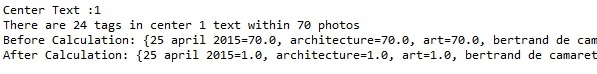
\includegraphics[width=50cm,bb=0 0 1820 73]{centroid.jpg}\vspace{-4ex}
	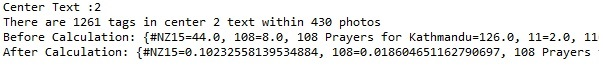
\includegraphics[width=50cm,bb=0 0 1820 73]{centroid2.jpg}\vspace{-4ex}
	\caption{Centroids Keywords from the appreciation}\label{fig:centroid}
\end{figure}

Given two weighted tag sets $A$ and $B$, their Jaccard-based tag similarity is defined as:
\begin{equation}\label{eq:JAAAAC}
 J_t(A,B) = \frac{\|A\cap B\|}{\|A\cup B\|} = \frac{\|A\cap B\|}{\|A\|+\|B\|-\|A\cap B\|}
\end{equation}


\noindent where the $\|A\|$ is the weighted number of tags in set $A$. Our $J_t$ measure can be used for the matching between images and that of image groups as well.

\eat{
The tags are attached to the images by the uploaders and may vary. As shown in Figure 2, the image tags use Jaccard Distance Similarity method to find the similarity between the tags. To make the tag similarity more accurate, we made one extend to the tags. We first weight the tags on images and then deploy a weighted version of Jaccard metric to measure the similarity between images. Specially, the tags assign with the value of 1 as a default, but when the centroids are calculated, the tags weight will be the average of the tags appears in the images. By using the weighted tags, we are able to see the texture differences between the centroids and the distances of the images tags. For the default tags, tag similarity distances can be calculate with the basic Jaccard similarity equation \cite{Jaccard},which is:
\begin{equation}\label{eq:JAAAAC}
 J(A,B) = \frac{|A\cap B|}{|A\cup B|} = \frac{|A\cap B|}{|A|+|B|-|A\cap B|}
\end{equation}


Where the `A' is the user input and the `B' is the tags. This equation calculates the distances between the user inputs and all the images tags.

Although, the tags similarities do have a certain accuracy, the human error issues are exist when the clustering algorithm only use the tags similarity as the data sets. This because the image tags could contain the unrelated tags. Therefore, to increase the accuracy of clustering we use the Location Distance Similarity.
\footnotetext{http://bit.ly/1XdoJ36}
\footnotetext[2]{http://bit.ly/1Uka1Fa}
}
\subsection{Location-based similarity(LDS)}

To detect changes from images, 
it is important to prevent gathering the images having the similar tags but different location. 
Thus, location information is vital here. 
The location of an image can be described as a pair of its latitude and longitude. 
We approximate the location of an group of $N$ images as a pair of average latitude and average longitude over the whole group, which can be computed by:
\begin{eqnarray}\label{equ:meanLocation}
Lat=\frac{1}{N}\sum_{i=1}^N Lat_i \\
Lon=\frac{1}{N}\sum_{i=1}^N Lon_i,
\end{eqnarray}
\yongli{Fixed some error here. Please double check these two equations are correct or not.}
where $Lat$ denotes latitude and $Lon$ longitude.

Since there are no straight lines on the sphere, 
we deploy the ``Great Circle Distance(GCD)" to calculate the distance between the images, which measures the shortest distance between two image locations on the surface of a sphere and can be computed by the Haversine Formula \cite{10.2307/2309088}. Let $a$ denote Haversine, and $c$ the great circle distance in radians. Then the location distance $D$ is computed by equations \ref{equ:d} (a)-(c).
\begin{eqnarray}\label{equ:d}
	a = sin²(ΔLat/2) + cos Lat1 ⋅ cos Lat2 ⋅ sin²(ΔLon/2)\\
	c = 2 ⋅ atan2(  \sqrt{a},  \sqrt{(1-a)} )\\
	D = R ⋅ c
\end{eqnarray}
\noindent where $R$ is earth's radius. As suggested by Johor et al. 2013~\cite{Standardization}, the location distances are normalised to remove the potential biases among different features. It has been proved that the ``Min-Max" standardization had the lowest error rate to $k$-means algorithms \cite{Standardization}. Thus, we exploit this technique for location distance normalization, which is computed by:
\begin{equation}
D' = \frac{D-min(D)}{max(D)-min(D)}
\end{equation} 	
\noindent where $D$ denotes the distance between images.
%Formula from Johor et al., 2013 \cite{Standardization}, In this formula `x' is representing the location distance. ``min(x)" and ``max(x)" is the shortest and farthest distances in the distance list.


\subsection{Social Image Similarity}

Once the tag similarity and location distance measures are defined, 
we define the overall social image similarity (SIS) by fusing the tag-based distance and location-based distance, 
which is as follows:
\begin{equation}
SIS = \frac{1}{D'+1} * J_{t},
\end{equation}
where$D'$ denotes the location distance and $J_t$ the tag-based similarity. 

The value of $SIS$ between two images will be in the range from 0 to 1. 
A larger $SIS$ value indicates a higher probability of the images being closer to each other.

\section{Change Detection Over Large Data Sets}\label{sec-algorithm}

In this section, we present the change detection algorithm from the large-scale social images, 
including how to identify the image pairs from the same source and how to detect the changes in images.

%Since there are large data sets can be retrieved from the social media, there are two approaches to improving our clustering performance in both speed and accuracy.

\subsection{Image Copy Detection}

This section presents how to effectively and efficiently identify the image pairs of the same source (same building or infrastructures etc). 
Many image copy detection approaches have been proposed and applied for various applications. 
However,  since each image may contain up to thousands of 36-dimensional local descriptors, 
directly deploying existing technique is obviously not suitable for large image databases due to the high time cost. 
To improve the efficiency of image copy identification, 
we propose a process of $SIS$-based clustering,
then deploy a PCA-SIFT-based matching over images in the same or neighboring clusters.

\subsubsection{SIS-based clustering}

Intuitively, images from the same source usually have similarity over the concept level. 
Thus it is reasonable to cluster social images based on their tag and location information, 
such that those in a single cluster or neighboring clusters will have high possibility of being from the same source. 
In this way, the identification of image copy pairs can be simplified as the comparison between images from same or neighboring clusters, 
which avoids the costly pair-wise image matching over the whole data collection. 
To do this, we need to find an efficient clustering technique that can be extended to our $SIS$ social image similarity as well. 
%Conventional clustering techniques include partitioning clustering, hierarchical clustering, overlapping clustering and subspace clustering. 
As we operate on large scale image database, the efficiency of clustering process is extremely important. 
Moreover, we only care about the similarity between images in each cluster, thus permit the overlaps between multiple ones. Thus, we extend the 2-means clustering algorithm that was initially proposed for $L_p$ distance for our $SIS$ similarity considering its low time cost as stated in \cite{DBLP:conf/sigmod/ShenZH05,DBLP:journals/tkde/ZhouZCSBT10}. 

Given an image collection, we conduct the clustering by three steps: 
1) for each image, we model its metadata as tag set and its location as a pair of latitude and longitude values;
2) we select two images with the lowest similarity as the cluster centres of two initial cluster from the current data collection. Each of the remaining images are assigned to the cluster that has the higher similarity with it. The centre points are recursively recalculated based on Equations \ref{equ:Centroid} and \ref{equ:meanLocation}, together with the images allocation to clusters based on their similarity, until the new generated centre points are stable;
3) finally, we recursively select a bigger cluster on which the second step is conducted, until the number of clusters reaches to a threshold $\kappa$.

In the social media images often there are more than 10 tags on each image and comparing these tags between the images one by one is time-consuming. 
String hashing has been applied in many applications for improving the system efficiency \cite{DBLP:conf/sigmod/ZhouCZCHW15}. 
Thus we improve our change detection efficiency by selecting a ``good'' hashing function class. 
To reduce the time expenses on tags comparison, we use the \textit{djb2} hash function techniques \cite{MartínezFE14},
which one of the best hash function techniques for the string data. 
In \textit{djb2} the hash values are populated by \textit{hash*33 + c}, 
where the hash is the long data and $c$ is the string character. 
Daniel J. Bernstein uses the magic number 33 to times the hash data, however, he did not explain why it works better than any other constants.
In our system, the \textit{djb2} is applied to all the images tags and the hash value is created for each tag. These hash values are used when the $J_t$ similarity is calculated. The first step is making the tags on the image $A$ and the image $B$ to the hash values, and then it compares the hash values of $A$ with those of $B$. Secondly, if the hash value of $A$ does not exist in that of $B$, it is considered as unmatched. As such the system does not need to compare all the string tags. This hashing reduces the total number of string comparison in the $J_t$ similarity.

\eat{
Para 1: how to choose cluster algorithm, and extend it to SIS similarity

Para 2: how to index social images for quick clustering
}

\subsubsection{PCA-SIFT-based matching} 

PCA-SIFT-based matching will be used for deciding if two image candidates are referring to the same objects. 
It will find the similarity between the objects. The main objects are the buildings, statues and other objects which are not moving. Also, the unrelated images selected by the PCA-SIFT algorithm will be removed. 
The removing occur when the images have the high $SIS$ similarity, but the images are not what the user want. The kept image pairs are passed to change detection stage for assessing if any damages had happened in a natural disaster.

We apply the OOS to the similarity calculation between the local descriptor sets of two images \cite{DBLP:journals/tmm/ZhaoNTW07}. 
Given two local interest descriptors, the similarity between them is measured by the $Cosine$ similarity between these two vectors. For two local interest points from two images, they are match pair candidate if the similarity between them is bigger than a threshold value. OOS further check if any one of these two points is the nearest neighbor of the other among all the descriptors of its image. If they are nearest neighbors of each other, they are a real matched pair. The final similarity between two images is calculated by the average similarity of all their matched pairs. To improve the local interest points matching, we use the LIP-IS index proposed in \cite{DBLP:journals/tmm/ZhaoNTW07} as well. All these ensure that effective and efficient PCA-SIFT-based matching is performed.

\subsection{Change Detection}

Change detection assesses the damages caused during disasters. Intuitively, two pictures to the same location point contains same buildings or other objects, each is described as a boundary. 
If there is no damage happened at this place, the object boundaries in two images match. 
Otherwise, if there exists boundary missing or unmatched from the before image to the after one, the damages could have be caused in the disaster. Therefore, in this section, we propose a new image object boundary modelling together with a novel boundary matching method, which are robust to different image transformations, rotations or editing, for effective change detection.

\subsubsection{Model image boundary}

Existing works model building shadow area boundaries \cite{turker2008building}, boundary shapes \cite{rs2051217} using the coordinates of each pixel falling on the boundary of objects in an image. 
However, these boundary modelling incurs low effectiveness of detection for social images because of the possible object changes with respect to the viewpoints, rotations, space shift etc. 
To address this issue, we propose a robust boundary representation, called \emph{relative position annulus} (RPA), 
which describe each boundary as an annulus of the difference of neighboring edge lengths. 
Specifically, we exploit sober edge detector to detect a number of boundaries in an image, 
since it can detect the emphasising edges while reduce the effect of noise edges. Given a boundary consisting of $m$ vertexes $\{v_1,...,v_m\}$, we represent the boundary as $\{d(v_1,v_2)-d(v_2,v_3),...,d(v_{m-2},v_{m-1})-d(v_{m-1}-v_m), d(v_{m-1},v_m)-d(v_m,v_1)\}$, where any element can be the start point while other points are ordered clockwise. As such, the RPA representation will be robust to object rotation, viewpoint change and space shift in social images.

\subsubsection{Matching boundaries}
As each image may contain multiple objects, each image is described as a set of relative position annulus of multiple boundaries. 
To assess the damages in a disaster, we need to do two steps matching: 
(1) the measure between two RPAs; 
(2) the measure between two images. 
To further reduce the influence of small noise objects, we only use the top $\kappa$ biggest boundaries for boundary comparison between two images.

Given two RPAs, $\mathcal{Q}: <q_1, q_2,...,q_m>$ and $\mathcal{D}: <v_1,v_2,...,v_{n}>$ , we measure the similarity between them by extending the DTW \cite{Berndt:1994:UDT:3000850.3000887} for our annulus representation. In the matching, we consider $Q$ as a series, and $D$ as a set of $n$ series, where each series in the set takes $v_i$ ($i=1,...,n$) as the start point of the boundary and the remaining ones are ordered clockwise. Denote the series to $v_i$ as $\mathcal{D}_i$, and its elements as $<v_1^i,...v_n^i>$, where $v_j^i=v_{((i+j-1)\pmod n)}$. Then the similarity between $\mathcal{Q}$ and $\mathcal{D}_i$ is measured by:

\begin{equation}
\begin{array}{l}
SRPA_i(\mathcal{Q}, \mathcal{D}_i)= \left\{ \begin{array}{l}
 0 \hspace{1.7 cm}m=m_1-1~ or~ n=n_1-1 \\
max\{ SRPA_i(\mathcal{Q}_{m-1},\mathcal{D}_{n-1})+Sim(q_m,v_n^i),  \\
 ~~~~~~~SRPA_i(\mathcal{Q}_{m},\mathcal{D}_{n-1}), \\
 ~~~~~~~SRPA_i(\mathcal{D}_{m-1},\mathcal{D}_{n})\} \hspace{0.7cm} otherwise
 \end{array} \right.
 \end{array}
\label{SRPA}
\end{equation}
where $Sim$ is the similarity between $q_m$ and $v_n^i$ computed based on $L_1$ distance:
\begin{equation}\label{Sim}
  Sim(q_m,v_n^i)=\frac{1}{1+|q_m-v_n^i|}.
\end{equation}

\noindent The final boundary distance is decided by finding the maximal DTW between $\mathcal{Q}$ and $\mathcal{D}_i$
\begin{equation}\label{OverallSRPA}
  SRPA=\max_{i=1}^n SRPA_i.
\end{equation}


\eat{
\subsection{Clustering Techniques and Improvement}

The idea of the clustering algorithms is to group the large datasets into the smaller groups. Always the data within the same group have the similar data than the data in other clusters.
The clustering allows the system to use the centroids as the references of the cluster, and by referencing the centroids the system does not have to analyse all the data in the data sets. By knowing which cluster should be analysed, it increases the speed performance. However, there are some issues or limits on the clustering methods, such as the clustering methods could not handle some attribute types, time complexity and etc \cite{Berkhin2006}.

Moreover, Cheung~\cite{Cheung20032883} found there are 3 drawbacks for the K-MEANS algorithm. One of the drawbacks is that when the initialized(random) point are far away from the other points, it will remove immediately without learning within the learning process\footnotemark[2]. This means if the centroid is far from most of the points, the centroid's dimension is different from the major points' dimensions. In this research, there is one approach done with using this learning attitude. The approach is to pre-make the second centroid at the farthest point from the first centroid. The steps are followed by initialize the first random centroid, calculate the distance between the centroid and the points, and choose the farthest point as the second centroid. This approach is done to reduce the cycle of learning process(updating centroids) so that the process will improve the speed performance. This can be done in this research because, the main purpose of using Recursive 2 MEANS algorithm is to find the related images in the data sets and remove the unrelated images.

\footnotetext{Layer is the complete learning processes(step 1-5) for the K-MEANS}
\footnotetext[2]{The process at updating the centroid(step 2-3)}

\yongli{I suggest to move all Recursive 2 means related stuff to Section 2, as this is not your contribution. And focus on the Hash index one, and emphasis why it works, and how it works, and how much improvement it achieves, while you are using it with the k-means method.}

%The traditional methods are categorised in two categorise, the \textit{Hierarchical clustering} and the \textit{Partitioning clustering}. The \textit{Hierarchical Clustering} combines the data into clusters. It has two types top-down and bottom-up. the advantage is this can be use in any attribute types.

%The \textit{partitioning clustering method} is learning the clustering directly. k-mean is one of the type. it produce N points and use them as the center point. the data will learn base on these center points. the advantage is it does not depend on the data ordering. This reduce the time cost for sorting the data.

The approach is to use a Hash Index technique to improve the data accessing speed.
In the social media images often there are more than 10 tags on each image and comparing these tags between the images one by one are time-consuming.
To reduce the time expenses on tags comparison, we used the \textit{djb2} hash function techniques. The \textit{djb2} is known as best hash function technique for the string data compares to other hash function. In \textit{djb2} the hash values are populated by \textit{hash*33 + c}, where the hash is the long data and c is the string character. Daniel J. Bernstein uses the magic number 33 to times the hash data, however, he did not explain why it works better than any other constants.
In our system, the \textit{djb2} is applied to all the images tags and the hash value is created for each tag. These hash values are used when the Jaccard Distance Similarity is calculated. The first step is making the tags on the ImageA and the ImageB to the hash values, and then it compares the ImageA hash values with ImageB hash values. Secondly, if the ImageA hash value does not exist in the ImageB hash value, it considers as a not match. So that the system does not need to compare all the tags values in the string. This hashing reduce the total number of String comparison in the Jaccard Distance Similarity.

\subsection{Using PCA-SIFT}

%In this section, the PCA-SIFT is not tested, but Yan et al., 2004 \cite{1315206} experimented and got the results, which showed that the PCA-SIFT had better performance in both accuracy and speed.

In this research, PCA-SIFT will use for two processes. Firstly, it will find the similarity between the objects.
The main objects are the buildings, statues and other objects which are not moving. Also, the unrelated images choose by the PCA-SIFT algorithm will remove.
The removing occur when the images have the Final Distance same or close, but the images are not what the user want.
Those removed images are used to calculate the error rates.
The second process is to detect the changes between the images if the images contain the similar objects. These process will be explained in detail at the ``Experiment" section.
\yongli{Please detail the two runs of PCA-SIFT, which is your work. ;}


\subsection{Datasets Issues and approaches}

As mentioned in Section 4,
the Recursive 2 MEANS algorithm uses the numeric data. So, the image features are modelled to numeric to measure the similarities between images.
However, the modelled data do not show the tags information and locations information
which causes a difficulty when the PCA-SIFT try to find the before and after images.
Therefore, it is needed to find the tags and the weighted tags in the centroids to see the texture differences between the centroids and the distances.
The tags in the centroids are the average of the tags within a cluster, which can be calculated with:
\begin{eqnarray}
CentroidKeyword = K_1(\frac{P_0+P_1..P_n}{n}),K_2(\frac{P_0+P_1..P_n}{n}) ...K_n(\frac{P_n}{n}),
\end{eqnarray}
where $P_n$ denotes the points, $K_n$ are the keywords and $n$ denotes the number of modelled data. If all the points in the cluster have the same keyword, the Keyword weight will be assign to 1.
\eat{\yongli{what does 'the data' refer to?}}
For example, assume there are 2 points where the point 1 contains 3 keywords and point 2 contain 5 keywords.\\
Point 1 Keywords = \{``earthquake",``apple",``happy"\}\\
Point 2 Keywords = \{``earthquake",``natural",``disaster",``apple",``Nepal"\}

\begin{eqnarray}\label{eq:pareto mle2}
&CentroidKeyword = earthqauake(\frac{P_1+P_2}{2}), apple(\frac{P_1+P_2}{2}),natural(\frac{P_1}{2}), \nonumber\\ &disaster(\frac{P_1}{2}), Nepal(\frac{P_1}{2})= earthqauake(\frac{1+1}{2}), apple(\frac{1+1}{2}), \nonumber\\
&natural(\frac{1}{2}),disaster(\frac{1}{2}),Nepal(\frac{1}{2}) .
\end{eqnarray}
\eat{\yongli{This equation is confusing. what is $V$?}}
For the above sample, the centroid between two points is
\begin{displaymath}
CentroidKeyword = earthquake(1), apple(1), natural(0.5), disaster(0.5), Nepal(0.5).
\end{displaymath}
 By finding the centroid tags, we are able to know the main tags tagged within the cluster.
Comparing the before and after images clusters with the weighted centroids tags, we are able to reduce the searching loop for before and after image clusters.
The figure 3, is the sample from the change detection application.


\begin{figure}[h]
	\centering
	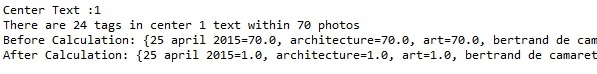
\includegraphics[width=50cm,bb=0 0 1820 73]{centroid.jpg}
	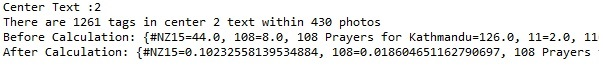
\includegraphics[width=50cm,bb=0 0 1820 73]{centroid2.jpg}
	\caption{Centroids Keywords from the appreciation}
	{\footnotesize Sample clusters tags data and weighted tags from application. Where the \textit{Center Text :1} is the first cluster and \textit{Center Text :2} is the second cluster. The line \textit{Before Calculation} and \textit{After Calculation} show the before and after the average calculation.}
\end{figure}

\pagebreak
}
\section{Experiment} \label{sec-evaluation}

In this section, 
we examine the performance of the proposed method,
focusing on its effectiveness and efficiency. 
Specifically, 
we answer:
\begin{itemize}
\item How does the proposed Social Image Similarity function perform? 
We answer this by investigate the efficiency of the SIS-based clustering models,
the effect of cluster numbers with different types of clustering techniques,
and the effect of hash index. 
\item How effective and efficient of the proposed boundary-based change detection method (\emph{BBCD})?
We compare \emph{BBCD} with existing state-of-the-art algorithms, the shape base change detection(\textit{SBCD})~\cite{rs2051217}. 
\end{itemize}

%
%We evaluate our proposed media sharing community image change detection approach in terms of effectiveness and efficiency. First, we evaluate the clustering model, which include the effect of cluster numbers, different types of clustering techniques and the effect of the hash index, to obtain the best before and after images match pairs. Then the effectiveness and the efficiency of our boundary based change detection(\textit{BBCD}) are evaluated using the best match pairs.  
%For each best match images, we compare our \textit{BBCD} with existing shape base change detection(\textit{SBCD}) \cite{rs2051217}. 
%\textit{BBCD} is using relative position annulus for image boundary, and the boundary of the buildings are developed in MATLAB. 
%Both change detection algorithms are using the overlap analysis to detect the changes, and for \textit{SBCD} without buffer was chose to use as an algorithm.

\subsection{Experimental Setup}

The dataset we experimented with is collected from Flickr
by focusing on images relevant to the \textit{Nepal earthquake}, which is also known as \textit{Gorkha earthquake}, in 2015.
Finally, 10,000 images are collected, which include images \emph{before} and \emph{after} the earthquake. 
The ground-truth is manually identified by the authors of this paper 
via careful comparison of all \emph{before} and \emph{after} images. 
Specifically, for a \emph{ground-truth}, 
both \emph{before} and \emph{after} image have to contain at least one same building,
but the corresponding image contents, angles, resolutions, colours and light effects could be different. 
This would allow the proposed method to analyse whether the before and the after images are taken in the same location and building. 

We conduct the efficiency experiments on 10000 after and before the earthquake images and their features. 4000 after and before the earthquake images are collected for the effectiveness experiment. 
\yongli{this is confusing. How many images you collected? 10000 + 4000? or the 4000 is in the 10000 actually? why do effectiveness only on 4000? for time reason?}

%These image collections are collected by using the Flickr APIs, and \textit{Nepal earthquake} also known as \textit{Gorkha earthquake} in 2015 was spotted as the main image resources. 
%Although it is impractical to browse all the images manually, due to the various image contents and the high noises, the ground-truth is manually identified by comparing all before and after the earthquake images. As a ground-truth, both before and after images have to contain at least one same building in the images, but the image contents, angles, resolutions, colours and light effects could be different. 
%This to allow the image matching algorithms to analyse whether the before and the after images are taken in the same location and building. 



\subsection{Measure metrics}


To evaluate the effectiveness of algorithms, 
we used two metrics in \cite{Zhou:2014:EDO:2628707.2628786}, 
the probability of miss detection and false alarm (\textit{Pmiss} and \textit{Pfa}). 
Specifically, the \emph{missed detection} mean that the algorithm fails to detect the ground-truth, and the \emph{false alarm} means the detection of non-target pairs. 
$Pmiss$ and $Pfa$ are defined as follows: 
\begin{equation}
Pmiss = \frac{number of missed detections}{number of ground truth}
\end{equation} 
\begin{equation}
Pfa = \frac{false alarms}{non targets }
\end{equation} 
a small value of \textit{Pmiss} and \textit{Pfa} means better effectiveness. 

The evaluation of efficiency includes two parts: 1) number of clusters, 
and 2) comparison with the existing damage detection algorithms.
Specifically, 
for number of clusters part test, 
it is expected to obtain the best cluster numbers to achieve the smallest \textit{Pmiss} and \textit{Pfa}.
We evaluate the efficiency of the proposed approach in terms of the overall time cost of clustering and hash index. 
We also evaluate the time cost of \textit{BBCD} and \textit{SBCD}, 
and to make the comparison more precise, we only compare the after the image matching time cost for change detection. 
Experiment are conducted on [machine information]...
\yongli{The above paragraph is very confusing, and please double check I rewrite what you want to present correctly. }

%Our aim for number of clusters part test is to obtain the best cluster numbers to achieve the smallest \textit{Pmiss} and \textit{Pfa}. The best cluster numbers will be used in the comparison with the existing technique. The effectiveness comparison part evaluates our \textit{BBCD} over other change detection techniques.


\subsection{Effectiveness}

We first examine the effect of number of cluster in \textit{SIS-based clustering} and \textit{OOS+LIP-IS}. 
After that, we compare the proposed approach with \textit{SBCD} by performing the change detection over the collected Flickr image datasets.

\subsubsection{Effect of clustering}

To examine the effect of the number of clusters $K$, 
we vary $K$ from 10 to 100 with a step length 10,
and for each cluster, 
it only looks for image pairs with 3 nearest neighbouring clusters. 
When calculating $Pmiss$, 
we only count the ground truth pairs that have more than 10 matches. 
%When calculating $Pfa$,
%for the non-ground truth pairs, 
%if the images containing the same objects but not choose as a ground truth will not be counted as a false alarm. 
The results are shown in Fig.~\ref{fig:HashFunction}.
It is observed that
1) when $K$ increases from 10 to 50, \emph{Pmiss} decreases from $0.35$ to $0.10$.
After that, \emph{Pmiss} starts increasing when $K > 50$ with slightly drop after $K > 80$. 
2) when increasing $K$, the overall trend of \emph{Pfa} is increasing,
which means more false alarms. 
But, there is a flat period for $Pfa$ is around $0.10$ when $K$ is between 40 and 60.
This may indicates $50$ is good candidate for the number of clusters. 

%We test the effect of the different number of cluster(\textit{K}) in effectiveness of the image matching, \textit{OOS+LIP-IS}. In this test, \textit{K} is varied from 10 to 100, and each clustered clusters only looked for their pairs with 3 nearest neighbour clusters. Also, we only count the ground truth pairs which have more than 10 matches between the images for the probability of miss detection.
%For the non-ground truth pairs if the images have taken same objects but not choose as a ground truth will not be counted as a false alarm. 
%As we can see the with increase of\textit{K}, the \textit{Pmiss} decrease gradually from 10 to 50, and reach to their bottom. With further increase of \textit{K} after 50, the effectiveness of  \textit{OOS+LIP-IS} increase. For the \textit{Pfa}, the increase of \textit{K} increases the false alarm. In both case, we can see the probabilities are not constant. This caused by two reasons. When our \textit{SIS-based clustering} fails to cluster the ground truth within the 3 nearest neighbours, \textit{OOS+LIP-IS} will pairs with no ground truth. Also, if there are several images, which took one part of the same building with ground truth, in some case \textit{OOS+LIP-IS} pairs with the non ground truth image too. 

\begin{figure}[ht!]\vspace{-4ex}
 \centering
       \scalebox{0.5}[0.5]{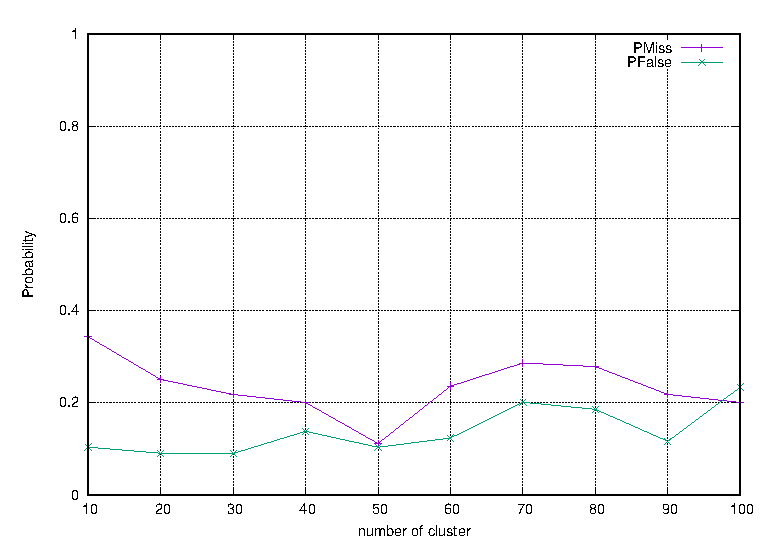
\includegraphics{PMPF.eps}}\vspace{-3ex}
    \caption{\small \vspace{-3ex} Hash and without hash time cost for number of cluster(\textit{K})\yongli{the title of this fig seems not right. It should be "The effect of the number of clusters". And the label for this fig is a duplicate of Fig.5. Please confirm which one is which. }}
     \label{fig:HashFunction}
\end{figure}

\subsubsection{Efficiency comparison}


\subsubsection{Comparing with existing technique}

comparing with shape-based approach. (in paper: \textbf{automatic detection of buildings and changes in buildings for updating of maps})

by varying the dataset size from small to big, test the probability of missed detection and probability of false alarm at each dataset size point

\eat{
\subsubsection{Effect of number tags : Effect of T}
\subsubsection{Effect of Cluster : Effect of K}
\subsubsection{comparison of EoT and EoK}
}

\subsection{Efficiency}

\subsubsection{Effect of different clustering techniques}

Here, we examine the efficiency of different clustering techniques when using them in the proposed change detection method. 
Specifically, 
we compare $K$-means and Recursive 2 Means 
by varying the number of cluster size from 5 to 100,
and then report the average time cost of building the clusters. 
The corresponding results are shown in Figure \ref{fig:Cluster}. 
It is observed that
1) when $K$ increases, the time cost increases for both techniques;
2) the time cost of $K$-means increases relatively quicker than Recursive 2 Means,
which means Recursive 2 Means is better.
%
%We evaluate the effect of clustering algorithms by varying the number of cluster size from 5 to 100 clusters with 5000 image dataset, and reporting the average time cost of  different clustering algorithms: (1)K-means; and (2)Recursive 2 Means for each clusters size. Figure \ref{fig:Cluster} shows the time cost change trends of two different approaches. As we can see when the number of cluster increase, the recursive 2 means perform better compares to k-means clustering.

\begin{figure}[ht!]\vspace{-4ex}
 \centering
       \scalebox{0.5}[0.5]{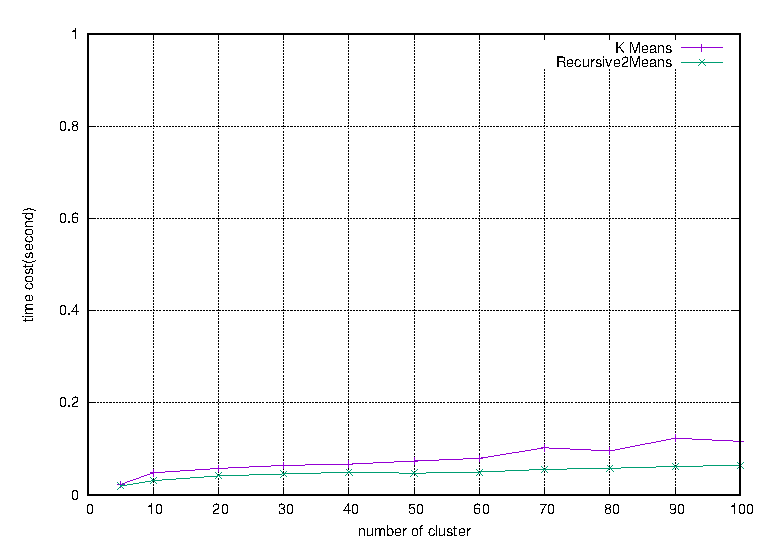
\includegraphics{ClusteringTimeCost.eps}}\vspace{-3ex}
    \caption{\small \vspace{-3ex} K-means and recursive 2 means clustering time cost}
     \label{fig:Cluster}
\end{figure}

\subsubsection{Effect of hashing index}

Now, we examine the efficiency of hashing index. 
Specifically, 
we compare the time cost of the proposed method with the \textit{djb2} hash function and without it. 
This is conducted over 1000 to 10000 images,
which is shown in Figure \ref{fig:HashFunction2}. 
It is observed that
1) the method of with hash function is significantly quicker than the counterpart of without hash function,
and the more the images, the larger the improvement. 
2) while the size of images increase from 1000 to 10000,
the time cost for the proposed method with hash function remain relatively small and stable;
however, the time cost of the counterpart without hash function increase over 7 times more. 
%
%we compare the time cost of \textit{djb2} hash function and without the hash function for our \textit{Tag-based Similarity} approach. The test conduct over 1000 to 10000 image dataset. Figure \ref{fig:HashFunction} compares our \textit{Tag-based Similarity} with the hash function \textit{djb2} in terms of the time cost used for similarity distance calculation.

\begin{figure}[ht!]\vspace{-4ex}
 \centering
       \scalebox{0.5}[0.5]{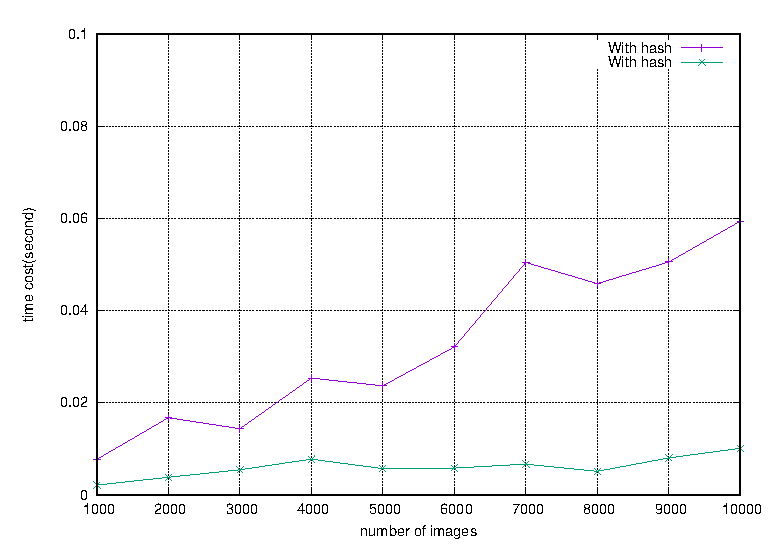
\includegraphics{JaccardTimeCost.eps}}\vspace{-3ex}
    \caption{\small \vspace{-3ex} Hash and without hash time cost for number of images\yongli{the legend of this fig is not right. }}
     \label{fig:HashFunction2}
\end{figure}
\subsubsection{Efficiency comparison}

Detection efficiency by varying data size

this is only for comparing our boundary-based approach and existing shape-based approach.

\section{Conclusion}\label{sec-con}
\bibliographystyle{ieeetr}
% there are various bibliography styles you can set

\bibliography{reference}
% this tells latex to generate the reference list, using the references.bib file of references.
% you will need to do pdflatex <tex filename>; then bibtex <tex filename without extension>;
% pdflatex <tex filename> again twice. then you have a formatted pdf.

\end{document}

